\chapter{The Node Controller}
\label{ch:controller}

\begin{defbox}[In this chapter you will learn]
\begin{itemize}
 \item the controller's per-millisecond loop, as an algorithm;
 \item the five states of the working-mode state machine, what each costs in charge and energy, and how states are chained;
 \item the start-up behaviour and the activation/shut-down hysteresis, from the code's point of view;
 \item the \emph{wait\_slot} state and its idealisations;
 \item the ``delivered-before-paid'' behaviour, measured: nearly half of the transmit states in the demo end in brown-out.
\end{itemize}
\end{defbox}

The \code{Controller} is the heart of a node. It owns the node's simulated \emph{behaviour}: it turns the capacitor voltage into duty-cycled activity (Chapter~\ref{ch:capacitor}), and activity into energy consumption and radio transmissions. Every node has one; each is a SimPy process that wakes up every millisecond.

\section{Configuration}

\codew{ControllerParams} bundles three frozen dataclasses (plus a maximum start-up time):
\begin{center}
\small
\renewcommand{\arraystretch}{1.12}
\begin{tabular}{@{}lrrrr@{}}
\toprule
State & Duration $d$ (ms) & Current $I$ (mA) & Charge $d\,I$ ($\si{\micro C}$) & Energy at $\SI{1.5}{V}$ ($\si{\micro J}$)\\
\midrule
listening & 5 & 0.14 & 0.70 & 1.05\\
sensing & 2 & 0.512 & 1.02 & 1.54\\
processing & 5 & 1.28 & 6.40 & 9.60\\
transmitting & 15 & 5.0 & 75.0 & 112.5\\
\midrule
\textbf{cycle} & 27 & -- & 83.1 & 124.7\\
\bottomrule
\end{tabular}
\end{center}
(demo values; the last column assumes a constant $\SI{1.5}{V}$). Transmitting is $90\%$ of the energy of a cycle. Thresholds are $\Vhigh=1.7$, $\Vlow=1.3$ \si{V}. \codew{max_startup_time_ms} (default $2000$) bounds a random start-up delay.

\begin{reality}[These demo loads are far from microwatt tags]
A transmit current of $\SI{5}{mA}$ at $\SI{1.5}{V}$ is $\SI{7.5}{mW}$, and the cycle averages $\SI{4.6}{mW}$. These are the electrical currents of a microcontroller-and-radio sensor node, three to four orders of magnitude above the $\sim\SI{1}{\micro W}$ class that 3GPP's first Ambient IoT release targets (Chapter~\ref{ch:intro}). They are parameters: nothing in the model prevents you from entering $\SI{1}{\micro A}$-class numbers, but the \emph{shipped demos} should not be read as representative of Ambient-IoT-class power.
\end{reality}

\section{The main loop}
\label{sec:ctlloop}

Algorithm~\ref{alg:ctlloop} is the \codew{Controller.run} generator in plain words.

\begin{algorithm}[t]
\caption{Controller main loop (every millisecond)}
\label{alg:ctlloop}
\begin{algorithmic}[1]
\State \textbf{each ms:} \quad publish \code{node.state}$\gets$ \code{state_name}
\State recompute harvest: \codew{calculate_node_power([node], downlink_results)} \quad \Comment{only if a map and results exist}
\State $\Vs\gets\sqrt{P_h\cdot R_s}$, \quad write to \codew{capacitor.voltage_source}
\If{\codew{capacitor.internal_time} $\le$ \codew{startup_delay}}
   \State interrupt capacitor with \texttt{charging}
\Else
   \State $v\gets$ \codew{capacitor.voltage}
   \If{$v\ge\Vhigh$ \textbf{and not} active}
      \State interrupt \texttt{full} (leak only); state$\gets$ listening; counter$\gets0$; active$\gets$ true
   \ElsIf{not active}
      \State interrupt \texttt{charging}; state$\gets$ listening
   \ElsIf{$v>\Vlow$}
      \State \Call{WorkingMode}{} \Comment{one FSM step; sets load and interrupts}
   \Else \Comment{$v\le\Vlow$ and active}
      \State active$\gets$ false; record FSM cycles of this charge cycle; interrupt \texttt{charging}
   \EndIf
\EndIf
\State \textbf{wait} 1 ms
\end{algorithmic}
\end{algorithm}

A few observations from the algorithm.
\begin{itemize}
 \item The \textbf{start-up delay} (uniform in $[0,2000)$~ms, drawn once per node) is measured on the \emph{capacitor's} own clock. During it the node charges even if $V$ already exceeds $\Vhigh$. Its purpose is to de-synchronise nodes that would otherwise all become active at the same simulated instant.
 \item \textbf{Activation} requires $v\ge\Vhigh$ \emph{and} the delay to have elapsed. At that moment the controller sends one \emph{leak-only} step (\texttt{capacitor\_full}), resets its state machine to \emph{listening} and sets the node active.
 \item \textbf{Shut-down} happens at the first millisecond where $v\le\Vlow$, \emph{wherever the state machine happens to be}.
 \item The voltage that the controller reads at step $k$ is the one produced by the capacitor update of step $k-1$ (Section~\ref{sec:onems}); the one-millisecond lag is harmless.
 \item The harvest power is recomputed in \emph{every} step: it changes when the node enters the \emph{transmitting} state (the $(1-\eta)$ rule of Chapter~\ref{ch:backscatter}) and with the solar trace.
\end{itemize}

\begin{reality}[The series resistance is not read from the capacitor]
Line~3 converts power to voltage using \codew{getattr(capacitor_ctrl, "R_series", 5e3)}. But \code{Capacitor} stores its resistance inside \code{params} (\codew{capacitor.params.R_series}); it has no attribute \code{R_series}. The \code{getattr} therefore \emph{always returns the default $\SI{5}{k\ohm}$}, whatever \codew{CapacitorParams.R_series} says. We verified this with a capacitor configured for $\SI{1}{k\ohm}$: \codew{hasattr(cap,"R_series")} is false and the lookup returns $5000$. In the shipped demos both values are $\SI{5}{k\ohm}$, so nothing goes wrong; if you change $R_s$ in \codew{CapacitorParams} without also changing the constant in \codew{Controller.run}, the equivalent source voltage and the capacitor's charging resistance will silently disagree.
\end{reality}

\section{The working-mode state machine}
\label{sec:fsm}

Once the node is active and $V>\Vlow$, each millisecond runs one step of the finite-state machine in Figure~\ref{fig:fsm}.

\begin{figure}[t]
\centering
\begin{tikzpicture}[>=Stealth,scale=0.95,transform shape]
 \node[st,fill=ablue!15,draw=ablue,minimum width=2.6cm] (L) at (0,0) {listening\\5\,ms, 0.14\,mA};
 \node[st,fill=agreen!15,draw=agreen,minimum width=2.6cm] (S) at (4.4,0) {sensing\\2\,ms, 0.51\,mA};
 \node[st,fill=apurple!15,draw=apurple,minimum width=2.6cm] (P) at (8.8,0) {processing\\5\,ms, 1.28\,mA};
 \node[st,fill=agold!40,draw=agold!80!black,minimum width=2.6cm] (W) at (8.8,-2.7) {wait\_slot\\no load, charging};
 \node[st,fill=ared!12,draw=ared,minimum width=2.6cm] (T) at (4.4,-2.7) {transmitting\\15\,ms, 5\,mA};
 \draw[->] (L) -- node[lab,above]{registered} (S);
 \draw[->] (S) -- (P);
 \draw[->] (P) -- (W);
 \draw[->] (W) -- node[lab,above,align=center]{slot valid:\\\code{do_transmit}} (T);
 \draw[->] (T.west) -| node[lab,pos=0.2,above]{done} (L.south);
 \draw[->] (L.north) -- ++(0,0.9) -| (12.3,-2.7) -- (W.east);
 \node[lab] at (6.2,1.12) {not registered: skip sensing and processing};
 \node[lab,align=center] at (4.4,-4.1) {if $V\le\Vlow$ in \emph{any} state the node switches off};
\end{tikzpicture}
\caption{The working-mode FSM. Numbers are the demo durations and currents. A node that is not yet registered skips sensing and processing (upper loop) and waits for a command (\emph{send\_id}) to give it a slot. A freshly registered node that has no sensor value yet returns from \emph{wait\_slot} to \emph{sensing} first.}
\label{fig:fsm}
\end{figure}

\paragraph{Mechanics common to all states.} A state is advanced by a \emph{counter} that increases by one each millisecond; the state ends when the counter reaches its configured duration. In every state except \emph{wait\_slot} the controller sets \codew{capacitor.current} to the state's current and sends the \texttt{charge\_and\_discharge} interrupt: the node \emph{draws} its load while the harvester \emph{charges} simultaneously.

\begin{description}[leftmargin=0.4cm,font=\sffamily\bfseries]
 \item[listening] ($d=5$): the receive window in the model's vocabulary. At its end a \emph{registered} node moves to \emph{sensing}; an unregistered one to \emph{wait\_slot}, where it can send its ID if a slot was offered.
 \item[sensing] ($d=2$): produces a sensor value (a random integer in $[100,255]$ in the stub); then \emph{processing}.
 \item[processing] ($d=5$): copies the sensed value to \codew{processed_data}; then \emph{wait\_slot}.
 \item[wait\_slot]: \textbf{draws no load and only charges}. Each millisecond the controller asks the protocol module whether a transmission is permitted now (\codew{controller_tx_ready}). If so, it \emph{immediately} calls \code{do_transmit}, records the data and moves to \emph{transmitting}.
 \item[transmitting] ($d=15$): draws $\SI{5}{mA}$ for $\SI{15}{ms}$; at the end the cycle count is incremented and the node returns to \emph{listening}.
\end{description}
Because \emph{wait\_slot} has no end condition other than a transmission (or the voltage dropping to $\Vlow$, impossible while no load is drawn and the harvester is charging), a node with nothing to say simply \emph{rests at full charge} until the base station gives it a slot. This is why the node-0 voltage in Figure~\ref{fig:sawtooth} climbs above $\SI{1.7}{V}$ during waiting.

\begin{reality}[Idealisations of \emph{wait\_slot}]
(i) Waiting draws \emph{zero} current. A real node must keep its wake-up receiver or timer alive: even $\SI{1}{\micro A}$ is not nothing. (ii) The listening state's ``receive window'' has no effect on whether commands are received (Chapter~\ref{ch:bsmodule}): commands are accepted in any state, including when the node is off.
\end{reality}

\section{One real energy cycle}
\label{sec:realcycle}

Figure~\ref{fig:fsmzoom} zooms into two transmissions of Node~0 from the broadcast demo ($\approx\SI{120}{ms}$), with the base-station slot structure underneath.

\begin{figure}[t]
\centering
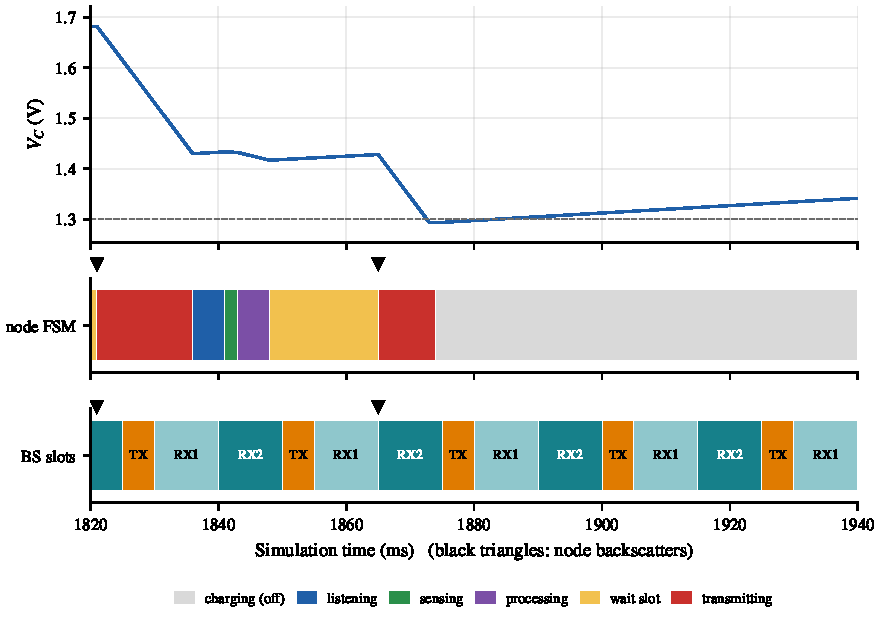
\includegraphics[width=\linewidth]{fig_fsm_zoom}
\caption{A $\SI{120}{ms}$ window of Node~0 (measured). Top: capacitor voltage; middle: the node's FSM state per millisecond (gold: waiting for a slot; grey: switched off and charging); bottom: the base station's frame (TX $\SI{5}{ms}$, two RX windows of $\SI{10}{ms}$). Black triangles mark the instants at which the node backscatters. Each packet is delivered at the \emph{start} of the node's transmit state, inside an RX window.}
\label{fig:fsmzoom}
\end{figure}

We can read off the entire mechanism.
\begin{enumerate}
 \item The first red bar is a full $\SI{15}{ms}$ transmit state: $V$ falls from $1.68$ to about $1.43$ V, i.e.\ $\Delta V=I\,T/C=\SI{0.25}{V}$ as predicted in Chapter~\ref{ch:capacitor}.
 \item Listening (blue), sensing (green) and processing (purple) follow, with a small drop each.
 \item During the gold \emph{wait\_slot} bar the voltage \emph{rises} (charge only). The wait ends at $\SI{1865}{ms}$, the first millisecond of the base station's next RX window in which the node holds a valid slot.
 \item The second transmit state starts, but $V$ reaches $\Vlow=\SI{1.3}{V}$ after only $9$~ms; the node \emph{switches off in the middle of its transmission}, and then charges (grey) for the next second.
\end{enumerate}

\begin{reality}[Delivered before paid]
The packet of the second transmission was handed to the base station at the first millisecond of the transmit state, \emph{before} the node paid the remaining $\SI{15}{ms}$ of energy. The controller's source says so explicitly: ``the \codew{transmitting} state \ldots\ only models the transmit energy draw; \ldots\ the reception has already happened.'' The consequence is energy \emph{causality}: nothing prevents a node from starting a transmission that its capacitor cannot finish, and it is still counted as delivered. We measured how often it happens in the shipped broadcast demo ($\SI{20}{s}$, one run): Node~0 had $25$ complete and $22$ truncated transmit states ($47\%$ truncated), Node~1 $9$ and $9$ ($50\%$), Node~2 $32$ and $24$ ($43\%$). Truncated states lasted only $9$--$\SI{11}{ms}$ instead of $\SI{15}{ms}$. A model in which a truncated burst counted as a \emph{lost} packet would report roughly half the throughput. This also explains the ``two packets per saw-tooth tooth'' of Chapter~\ref{ch:capacitor}. The design rule of that chapter applies: choose $C$, $\Vhigh$ and $\Vlow$ so that the energy window covers a full burst, or add a minimum-start voltage check before entering \emph{transmitting}.
\end{reality}

\section{Bookkeeping and logging}

\begin{itemize}
 \item \codew{fsm_count_in_current_cap_cycle} counts \emph{completed} FSM cycles (incremented at the end of \emph{transmitting}); on each shut-down it is appended to \codew{fsm_counts_per_cap_cycle}. In the demo these lists contain mostly $1$s, which is the footprint of the truncated second transmission above.
 \item \codew{data_history} records \codew{(capacitor time, value)} for every delivered datum of a registered node.
 \item \codew{acc_current_*} lists store the current of every step per state when \codew{keep_logs=True}.
 \item \codew{keep_logs=False} suppresses all per-step lists (flat memory for long runs).
\end{itemize}

\begin{codemap}
\small
\begin{tabularx}{\linewidth}{@{}>{\ttfamily}p{5.0cm}X@{}}
\toprule
\normalfont\bfseries Concept & \normalfont\bfseries Code (\file{controller.py})\\
\midrule
Currents, durations, thresholds & \codew{ControllerParams} (\code{CurrentsA}, \code{DurationsMs}, \codew{VoltageThresholdsV})\\
Main loop & \codew{Controller.run}\\
State machine & \codew{Controller.working_mode}\\
Charge-and-discharge request & \codew{Controller._enter_charge_and_discharge}\\
Registered? & \codew{Controller._is_registered}\\
Start-up delay & \codew{startup_delay_s}, from \codew{max_startup_time_ms}\\
\bottomrule
\end{tabularx}
\end{codemap}

\section{Chapter summary}
\begin{itemize}
 \item The controller wakes every ms, recomputes harvest, applies hysteresis and steps a five-state FSM; each active state draws its current while charging.
 \item A cycle costs $\approx83\,\si{\micro C}$, $\approx125\,\si{\micro J}$ at $\SI{1.5}{V}$, $90\%$ in the transmit state.
 \item \emph{wait\_slot} idles for free and charges; a node can rest above $\Vhigh$ indefinitely.
 \item Packets are delivered at the \emph{entry} of the transmit state; in the demo $43$--$50\%$ of transmit states are cut short by brown-out.
 \item The controller's conversion $\Vs=\sqrt{P_h R_s}$ always uses $R_s=\SI{5}{k\ohm}$, not the capacitor's parameter.
\end{itemize}

\section*{Exercises}
\begin{exercise}
Compute the energy of one FSM cycle at $\SI{1.7}{V}$ and at $\SI{1.3}{V}$ (charge is the same). By how much does the cycle's energy cost depend on the voltage at which it is run?
\end{exercise}
\begin{exercise}
A node is at $\SI{1.35}{V}$ when it enters \emph{transmitting}. Ignoring harvest and leakage, how long can it transmit before $\Vlow$? Express as a fraction of the $15$~ms burst. What minimum entry voltage guarantees a complete burst?
\end{exercise}
\begin{exercise}
Propose a one-line change to \code{wait_slot} that prevents transmissions from starting when the capacitor cannot complete them. What effect on throughput and on ``delivered'' statistics would you expect?
\end{exercise}
\begin{exercise}
Explain why the start-up delay is needed, and what the demo's collision statistics would look like for $N$ nodes if every node had a delay of zero and identical parameters.
\end{exercise}
